\documentclass[11pt,epsf,times,letterpaper]{article}
\usepackage[spanish]{babel}
\usepackage[latin1]{inputenc}
\usepackage{amsmath}
\usepackage{graphicx}
\usepackage{array}
\usepackage{enumerate}

\begin{document}

	\section{Ordertypes que minimizan}
	
	\begin{figure}[!h]
		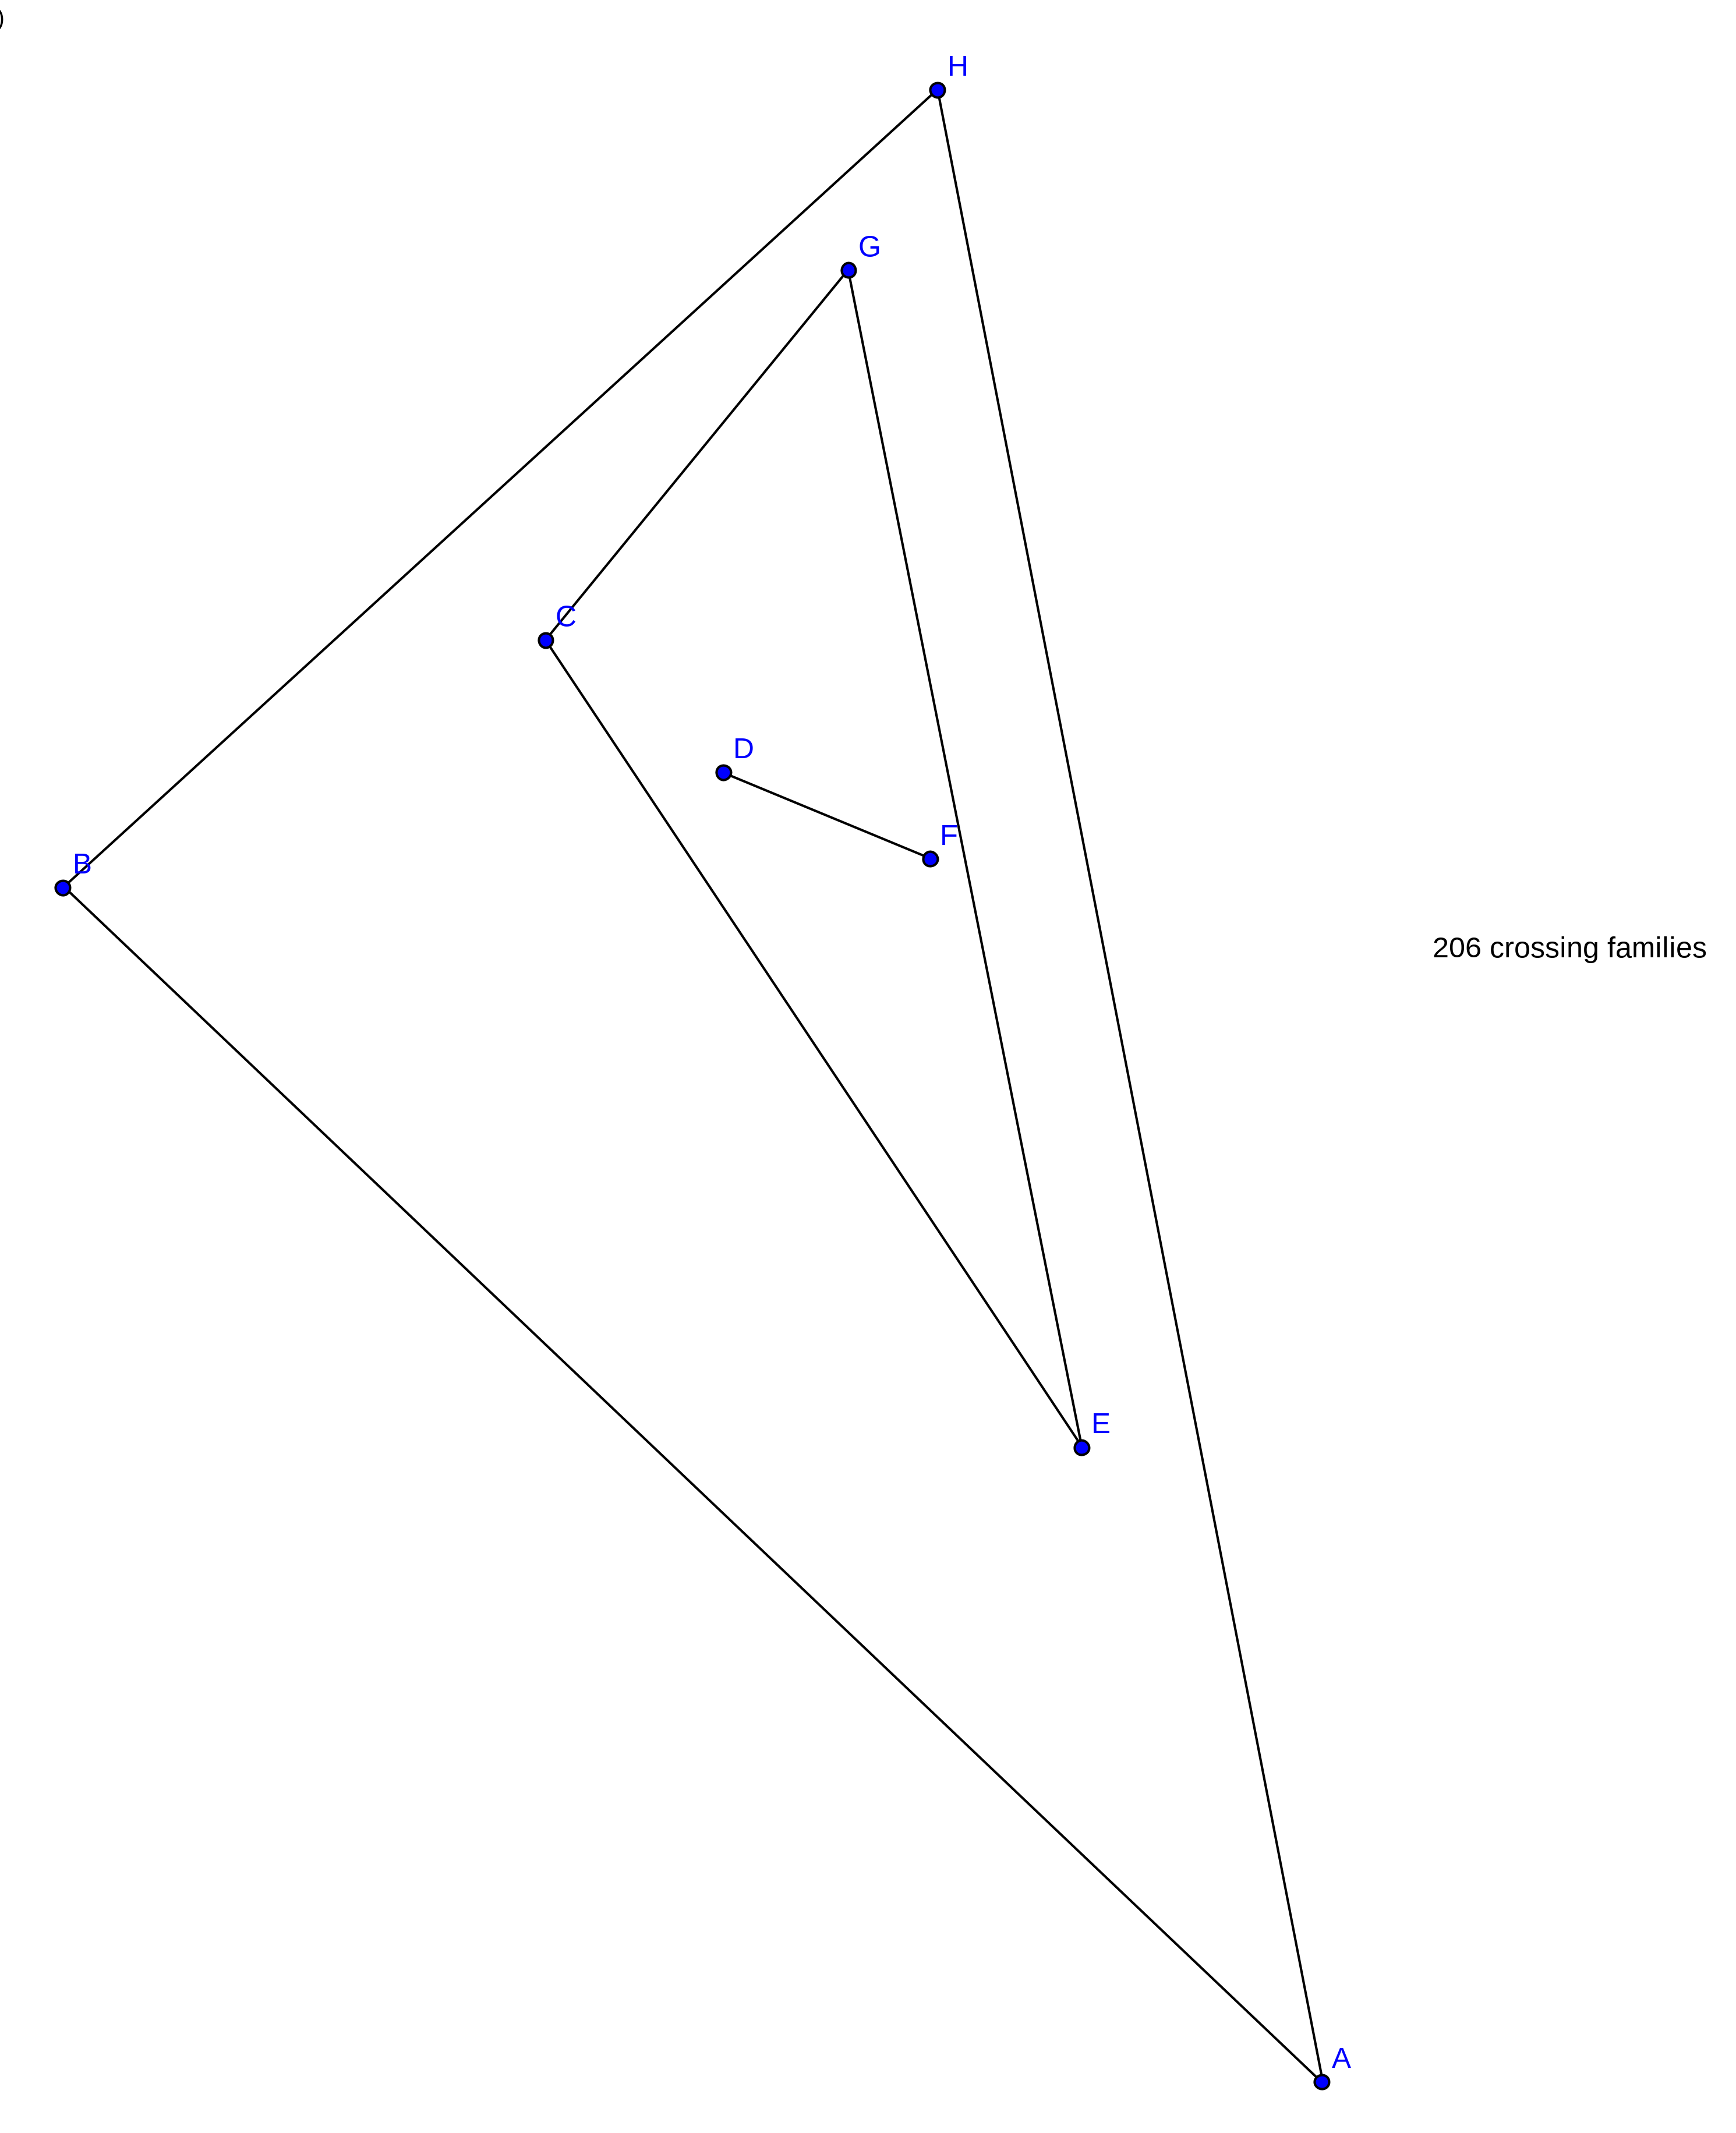
\includegraphics[scale=.25]{2k2/min8_otype2988.png}
		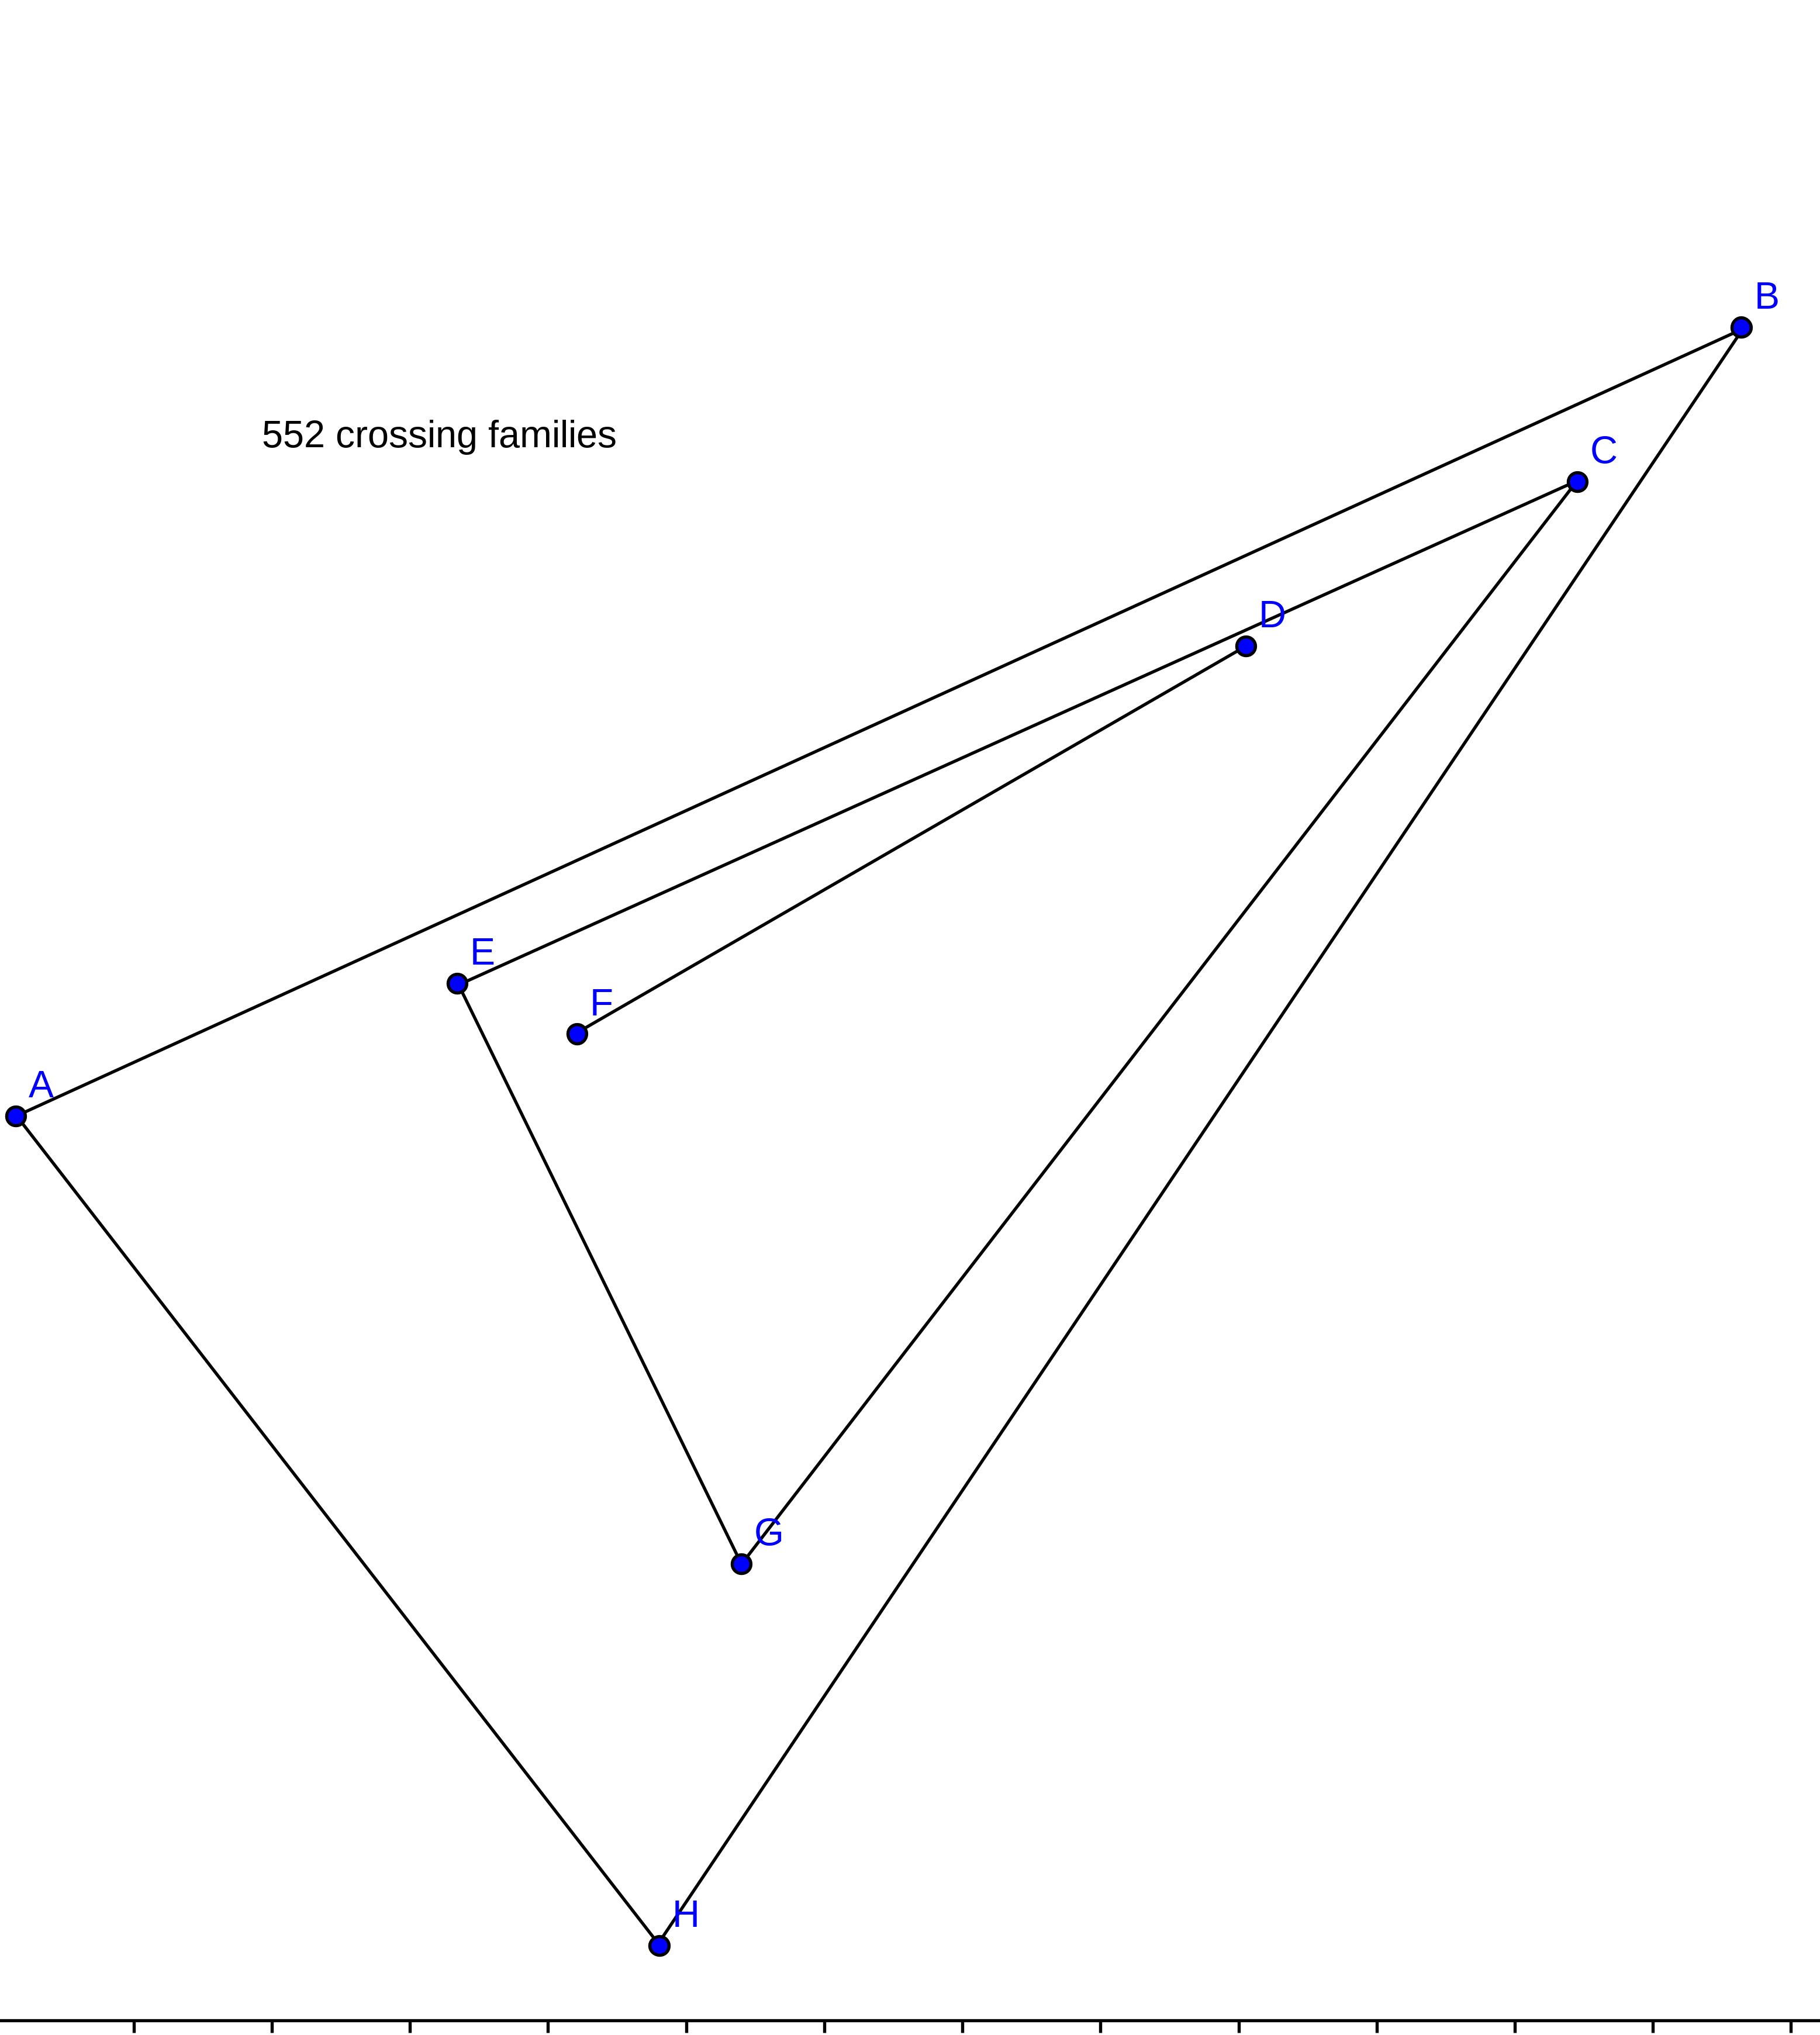
\includegraphics[scale=.25]{k13/min8_otype2991}
		\caption{otype 2988 para $2k2$ y otype 2991 para $k_{1,3}$ con 8 puntos}
				
	\end{figure}

	\begin{figure}[!h]
		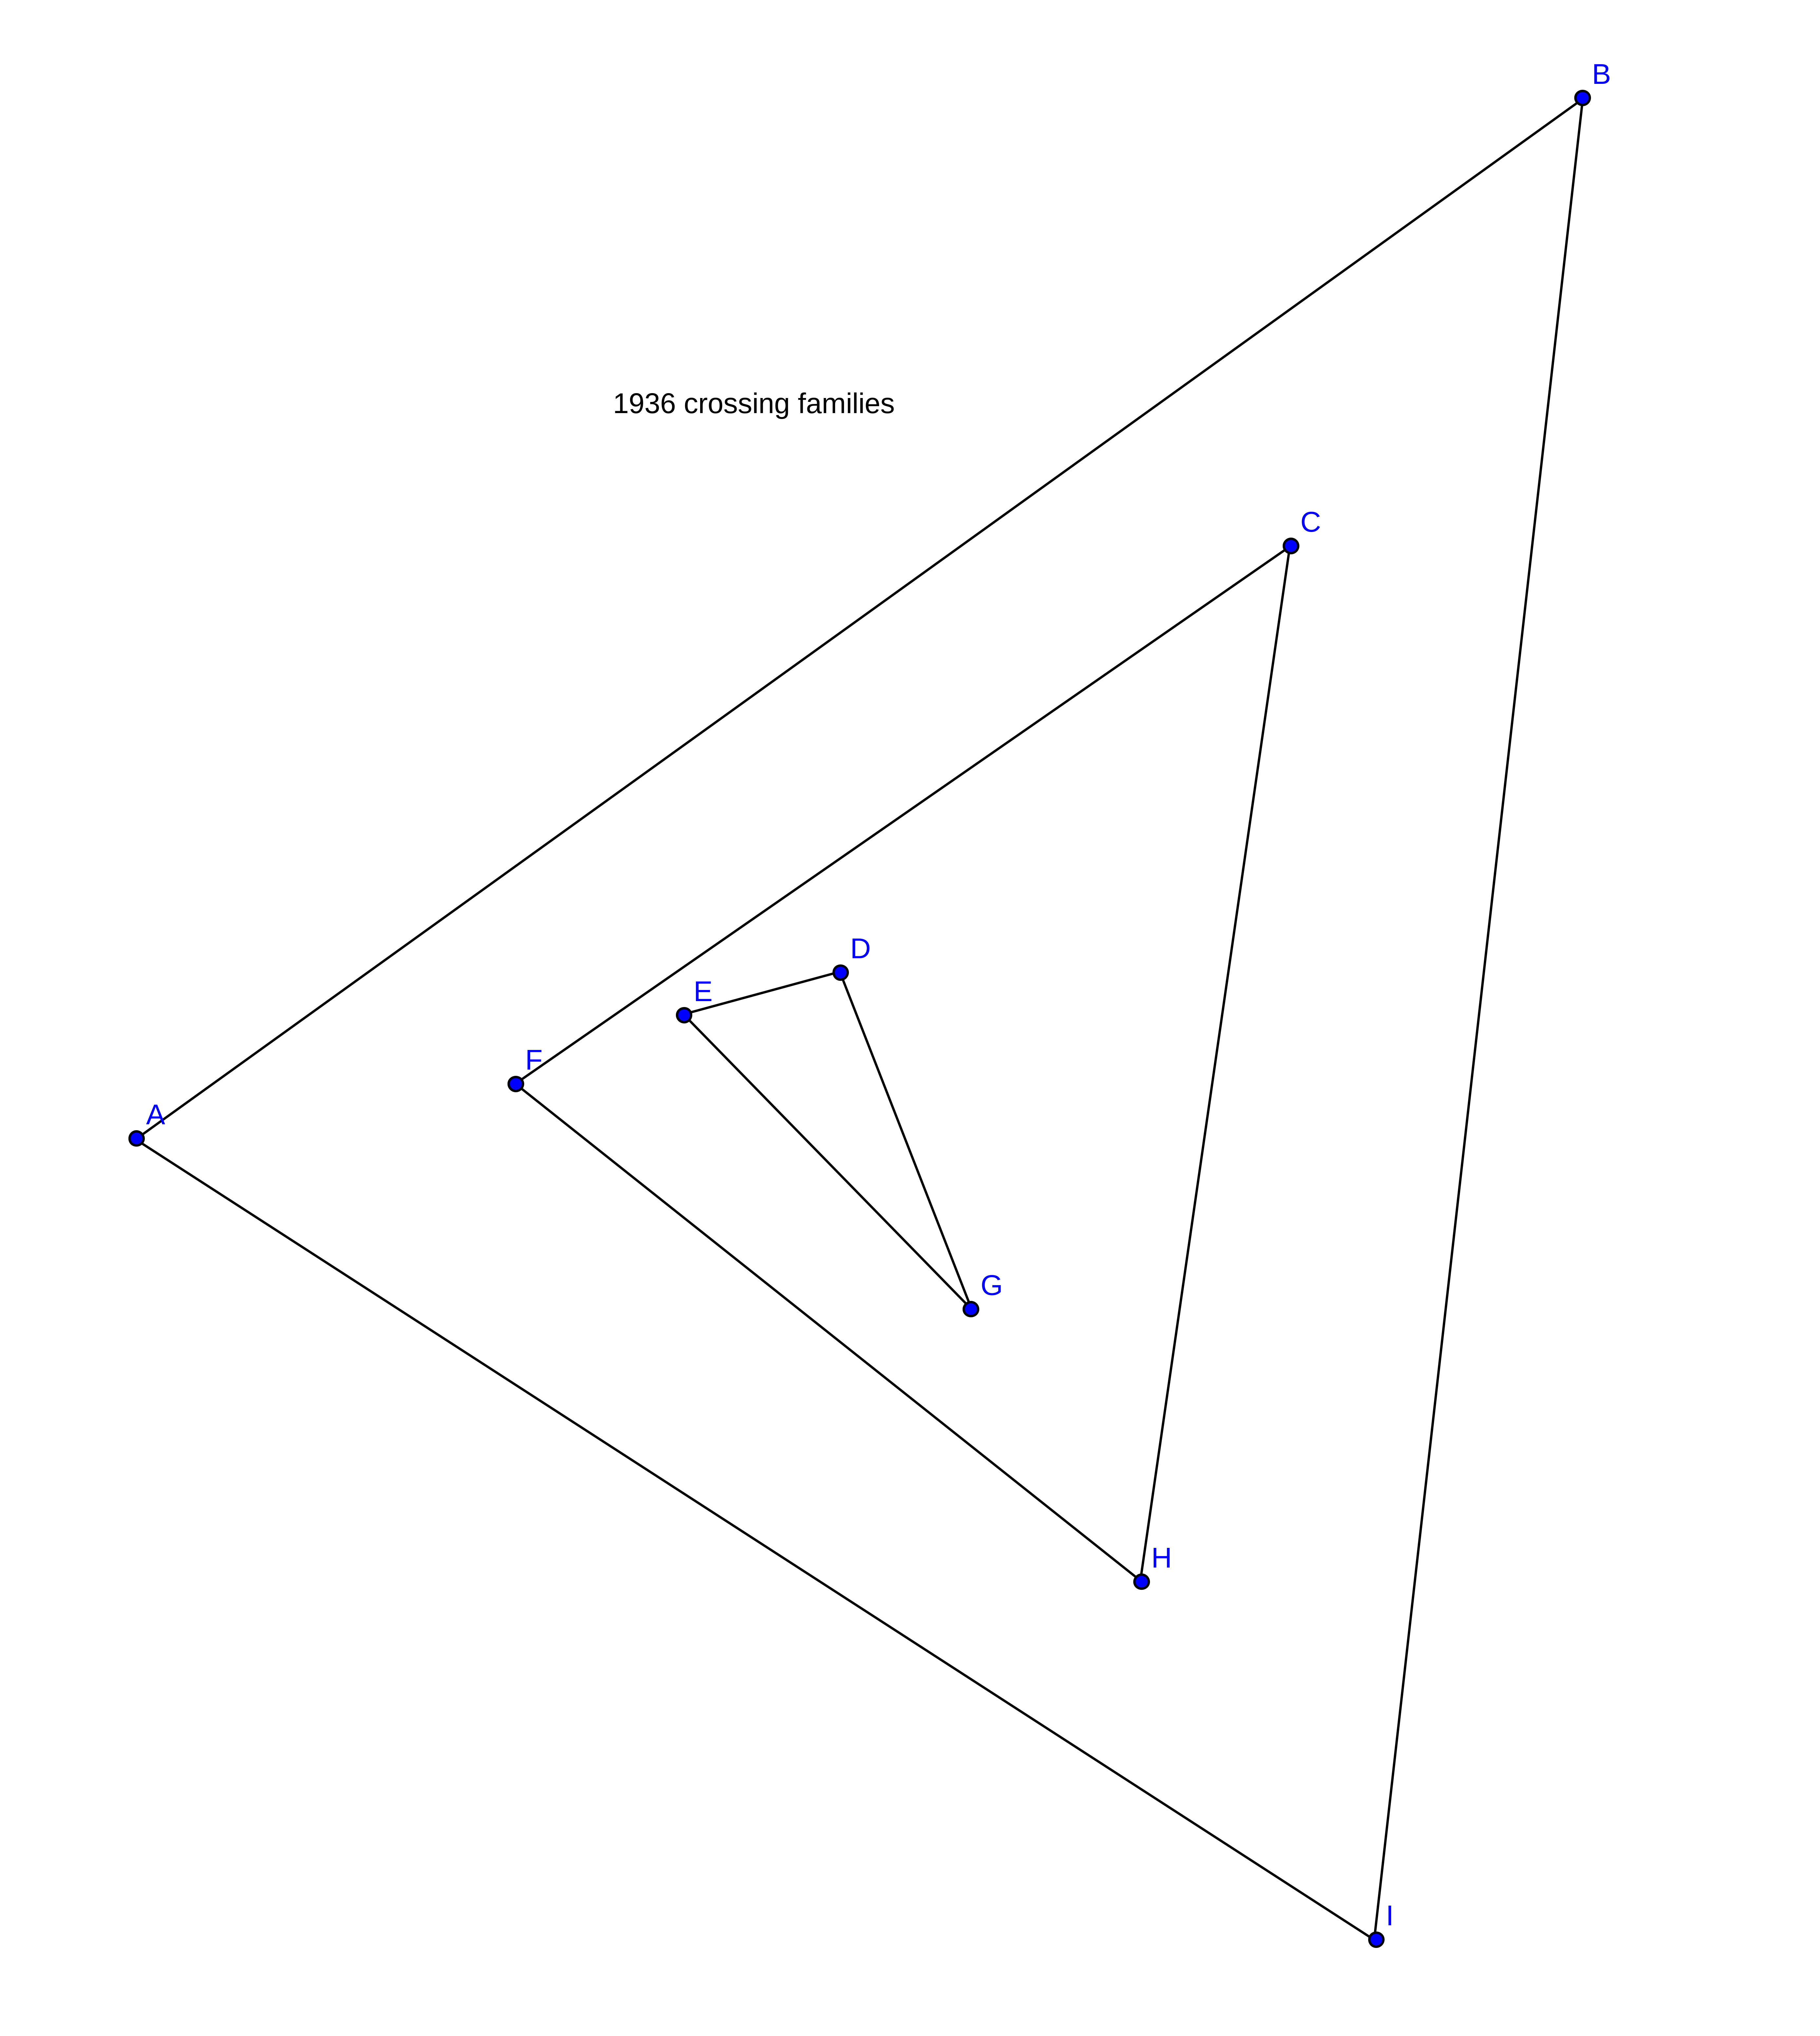
\includegraphics[scale=.125]{2k2/min9_otype151153.png}
		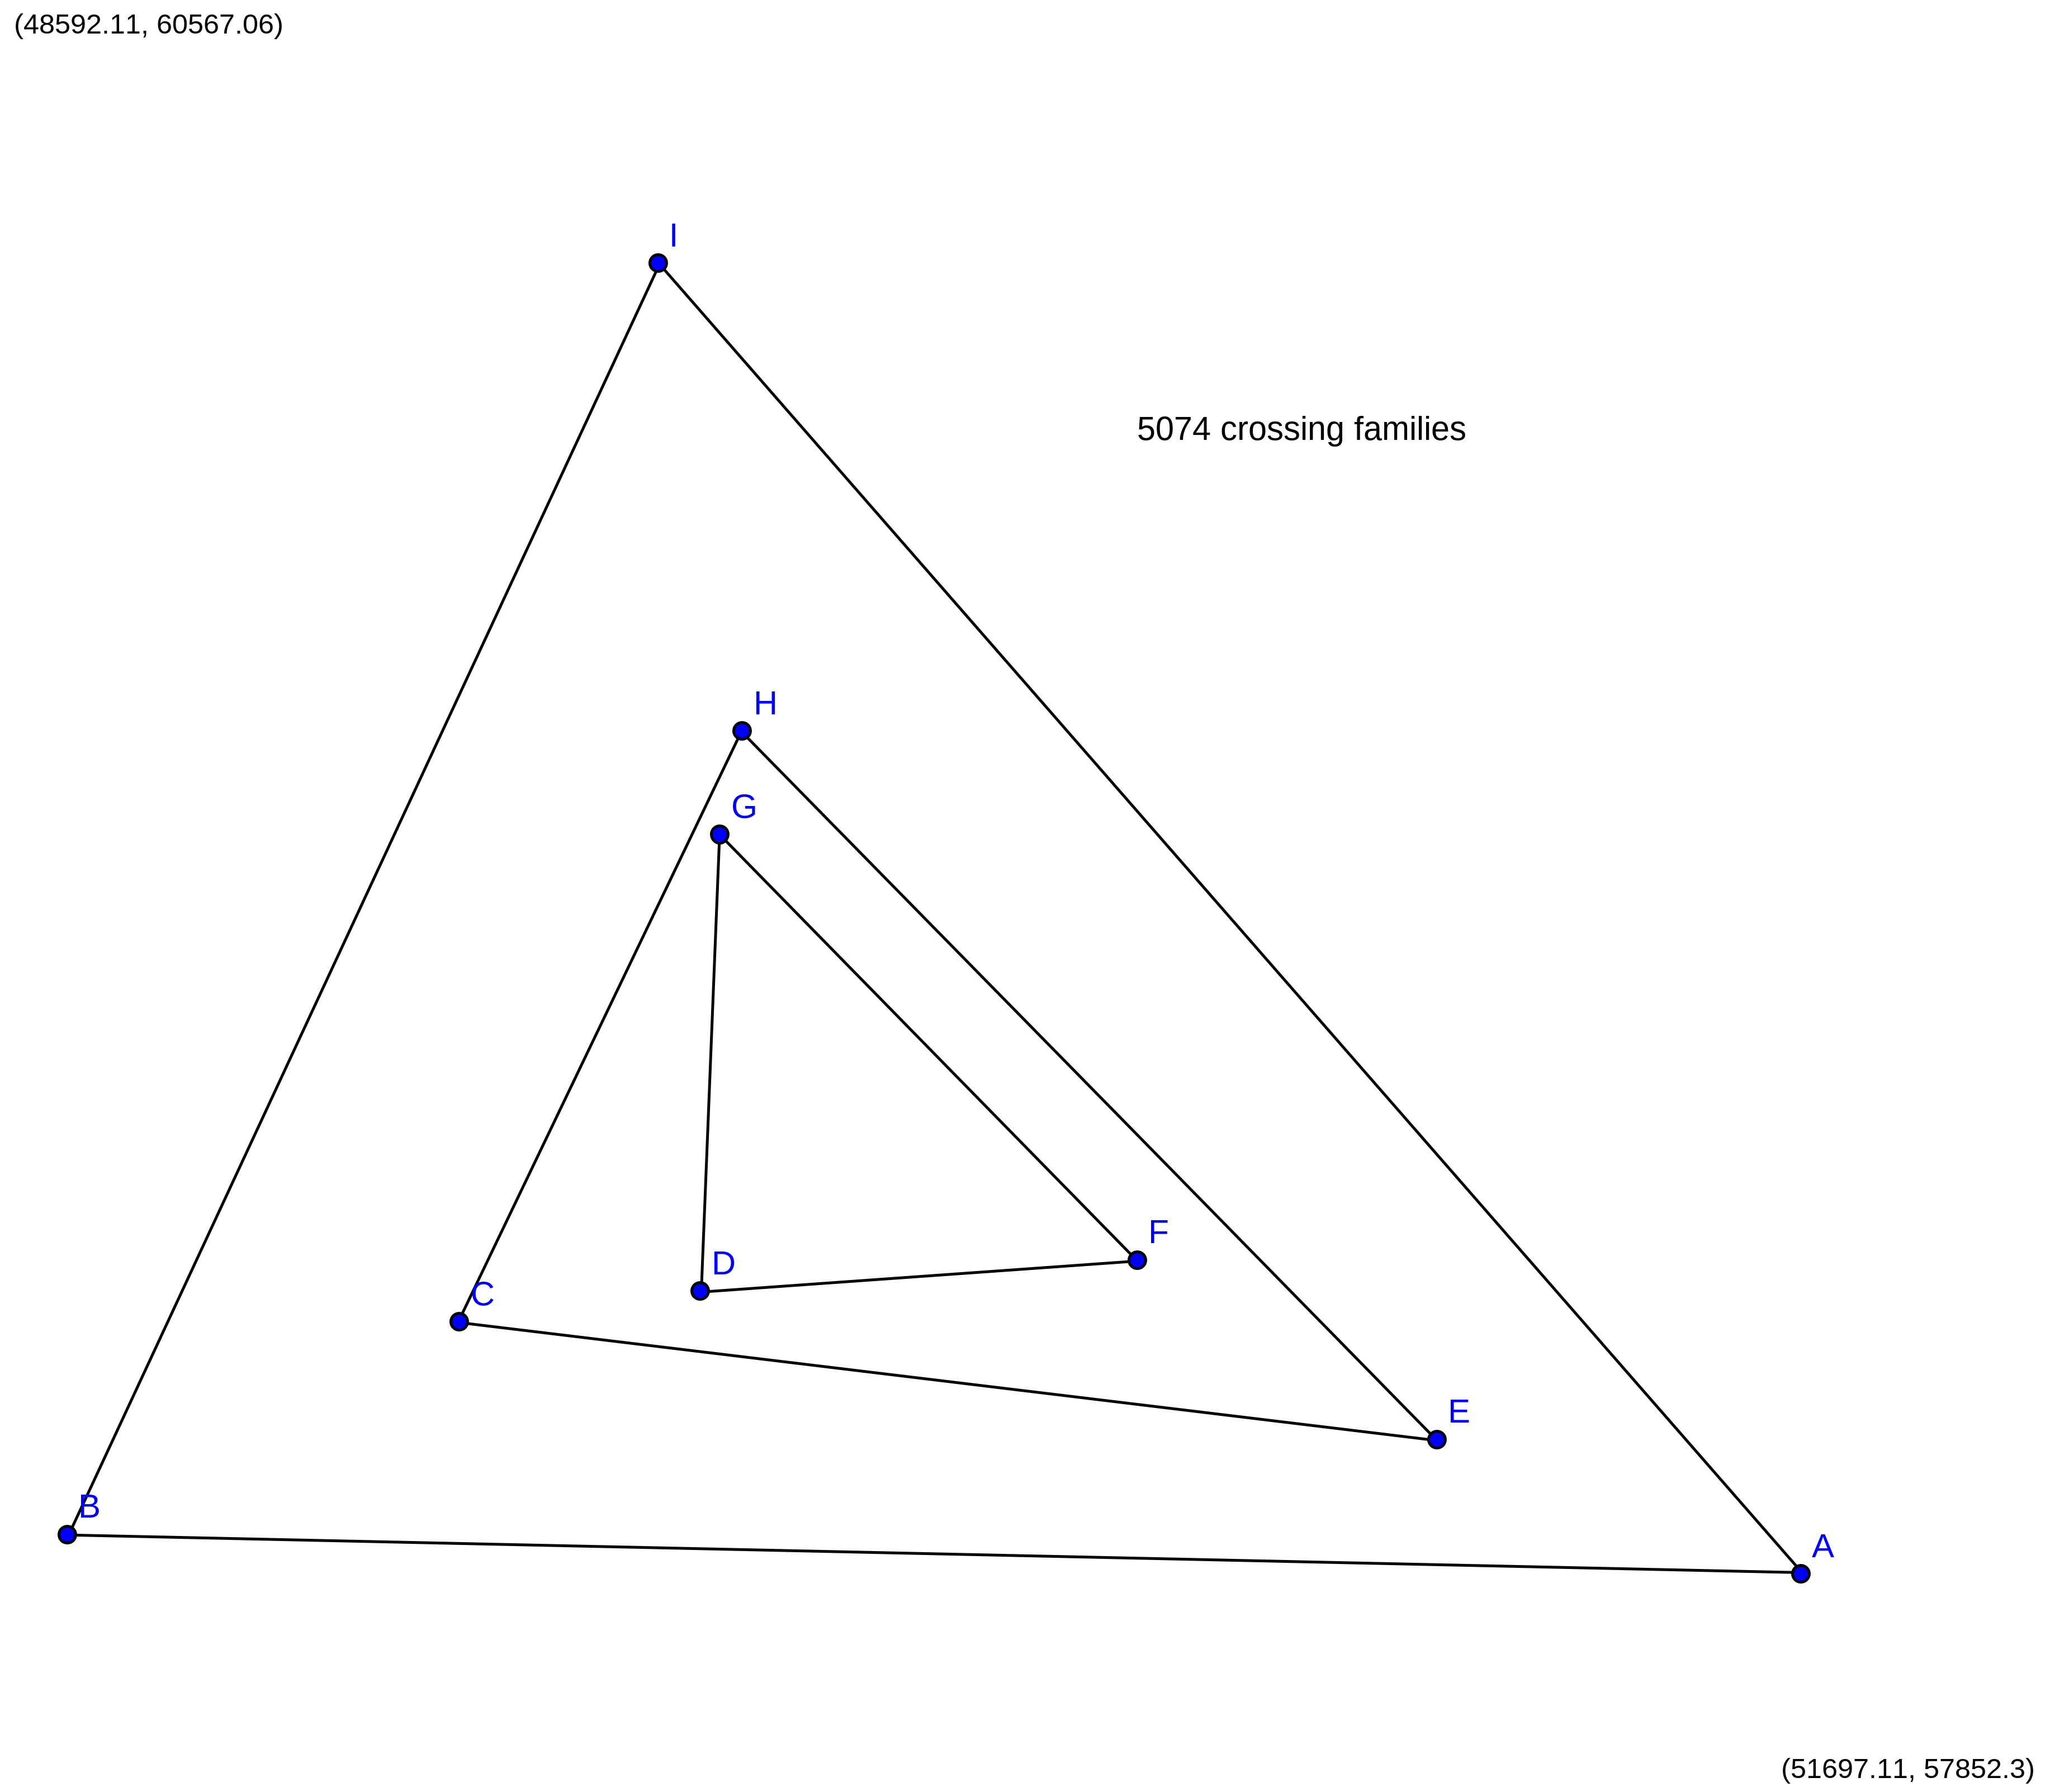
\includegraphics[scale=.25]{k13/min9_otype151720.png}
		\caption{otype 151153 para $2k2$ y otype 151720 para $K_{1,3}$ con 9 puntos}
	\end{figure}	

	\begin{figure}[!h]
		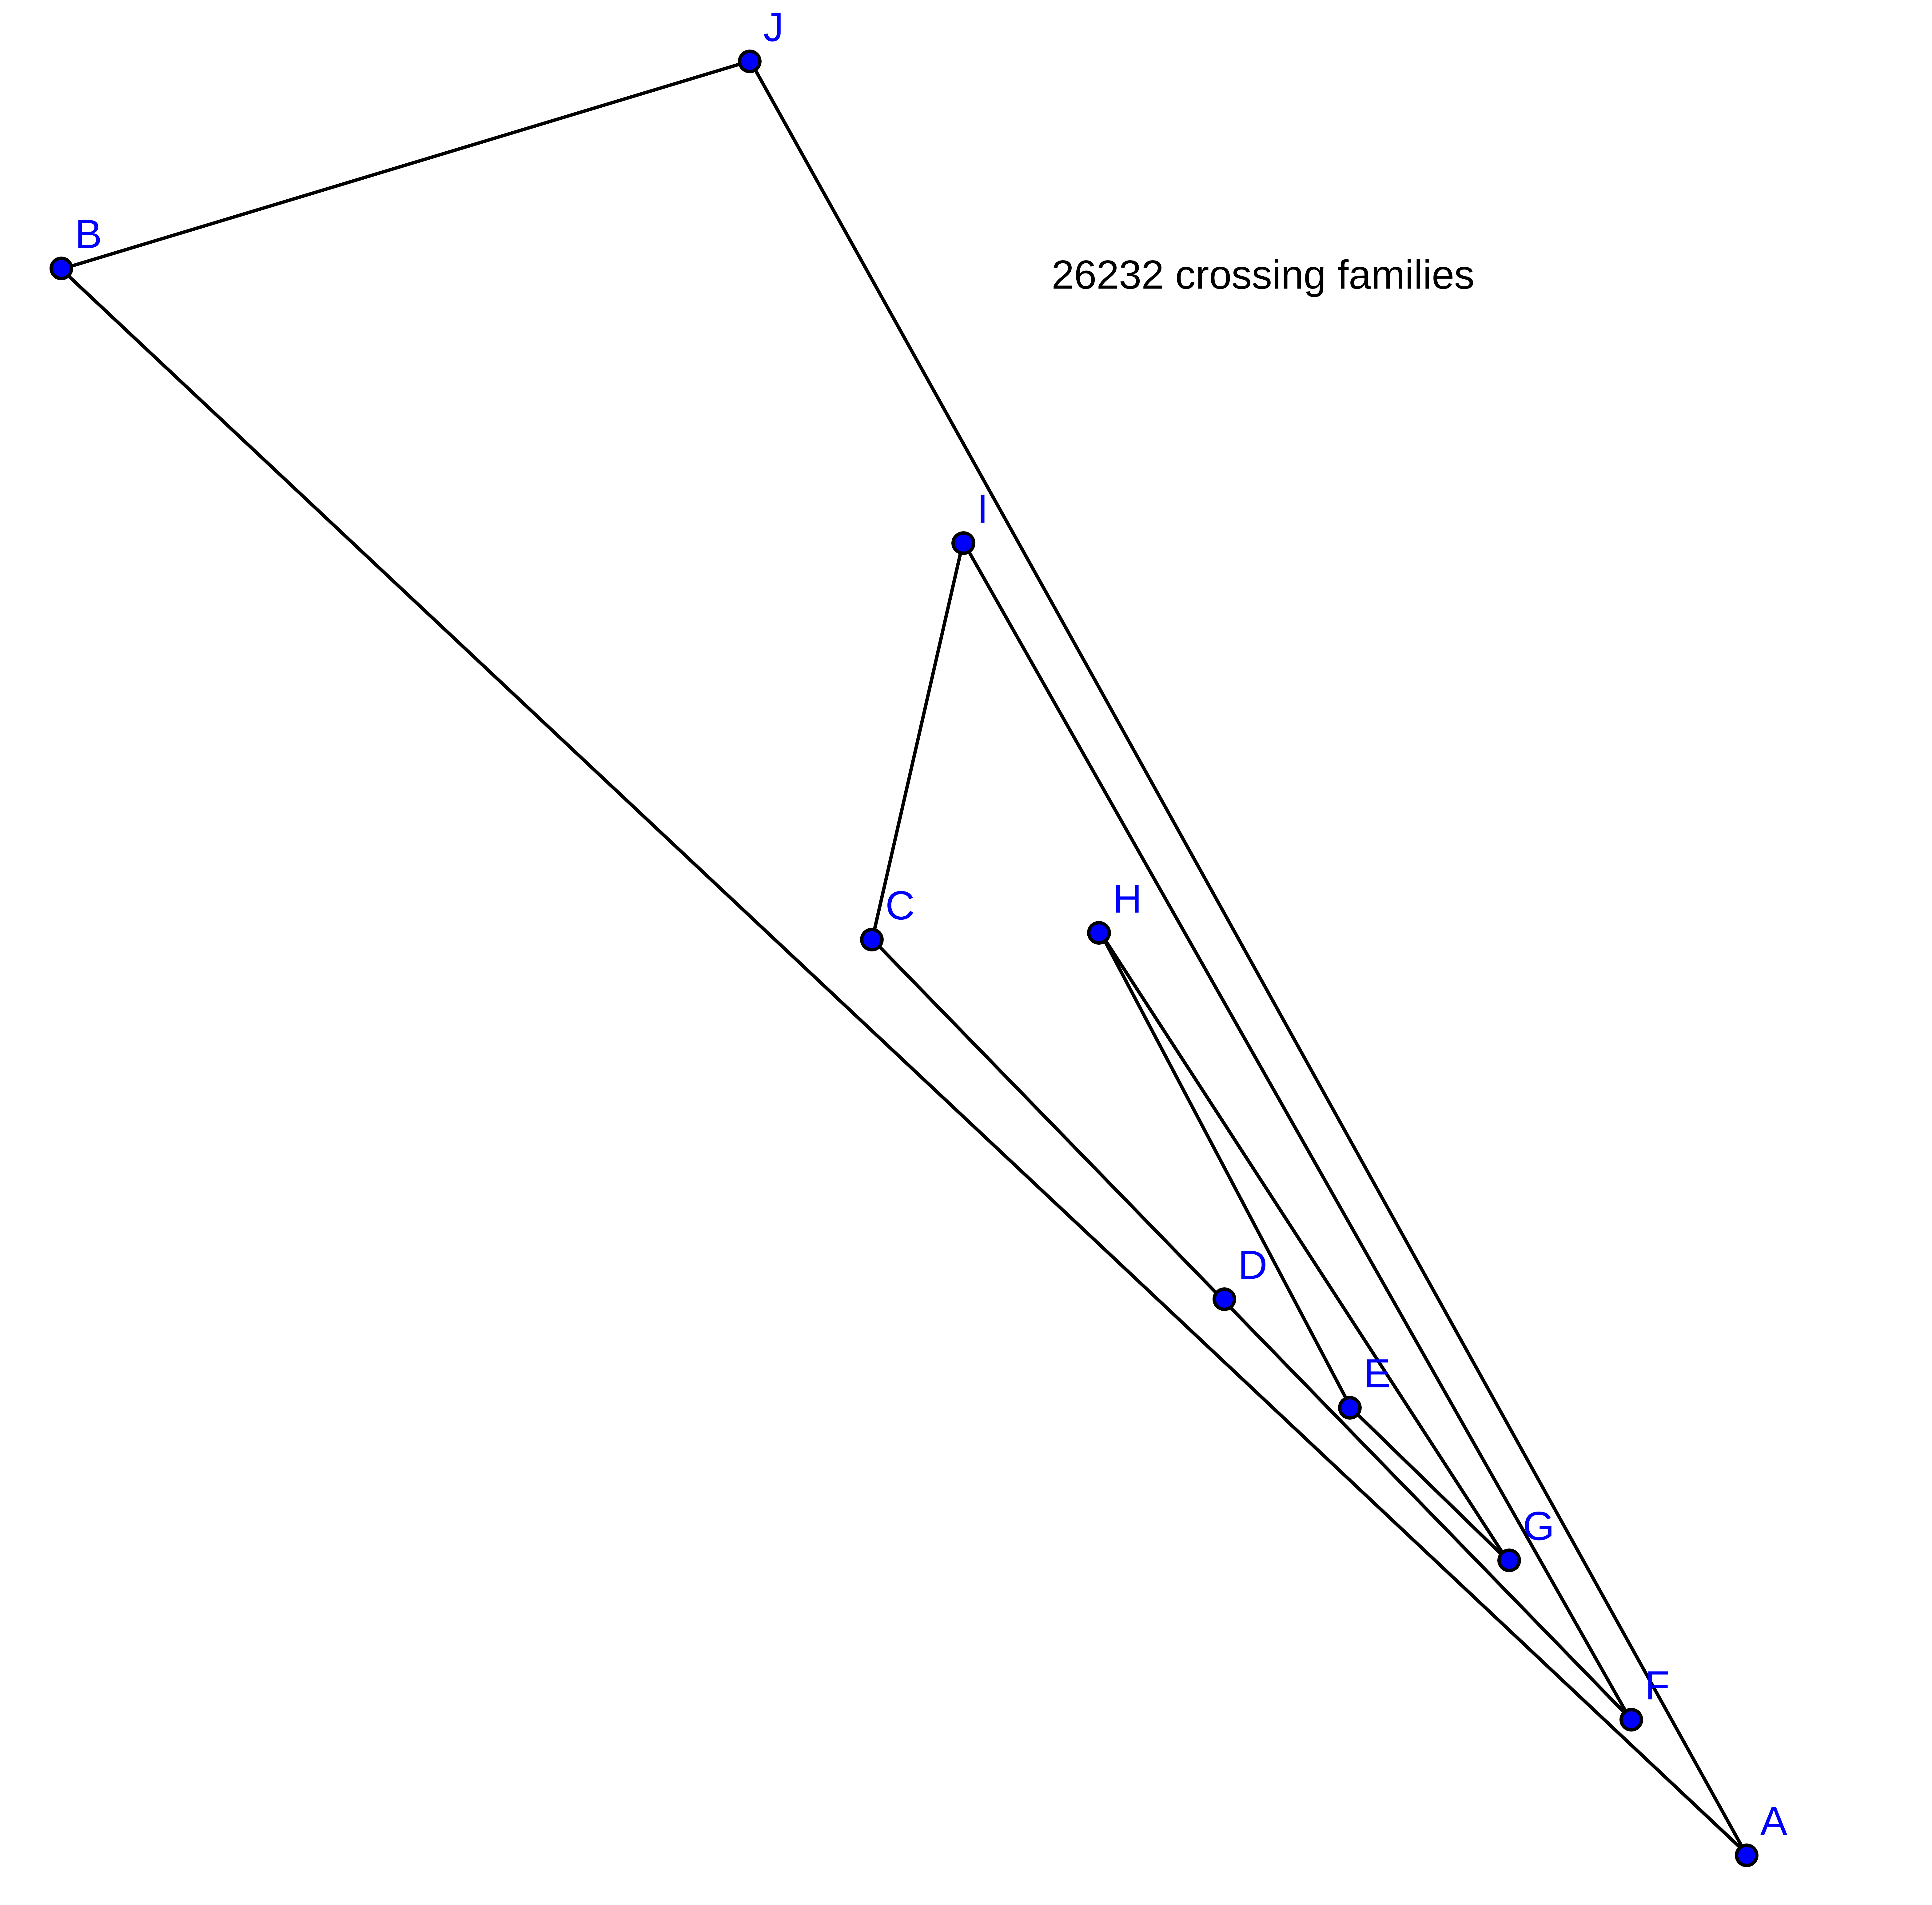
\includegraphics[scale=.25]{k13/min10_otype13468996.png}
		\caption{otype 13468996 para $K1_3$ con 10 puntos}
	\end{figure}

	\newpage
	\newpage

	\section{Ordertypes que maximizan}
	
	\begin{figure}[!h]
		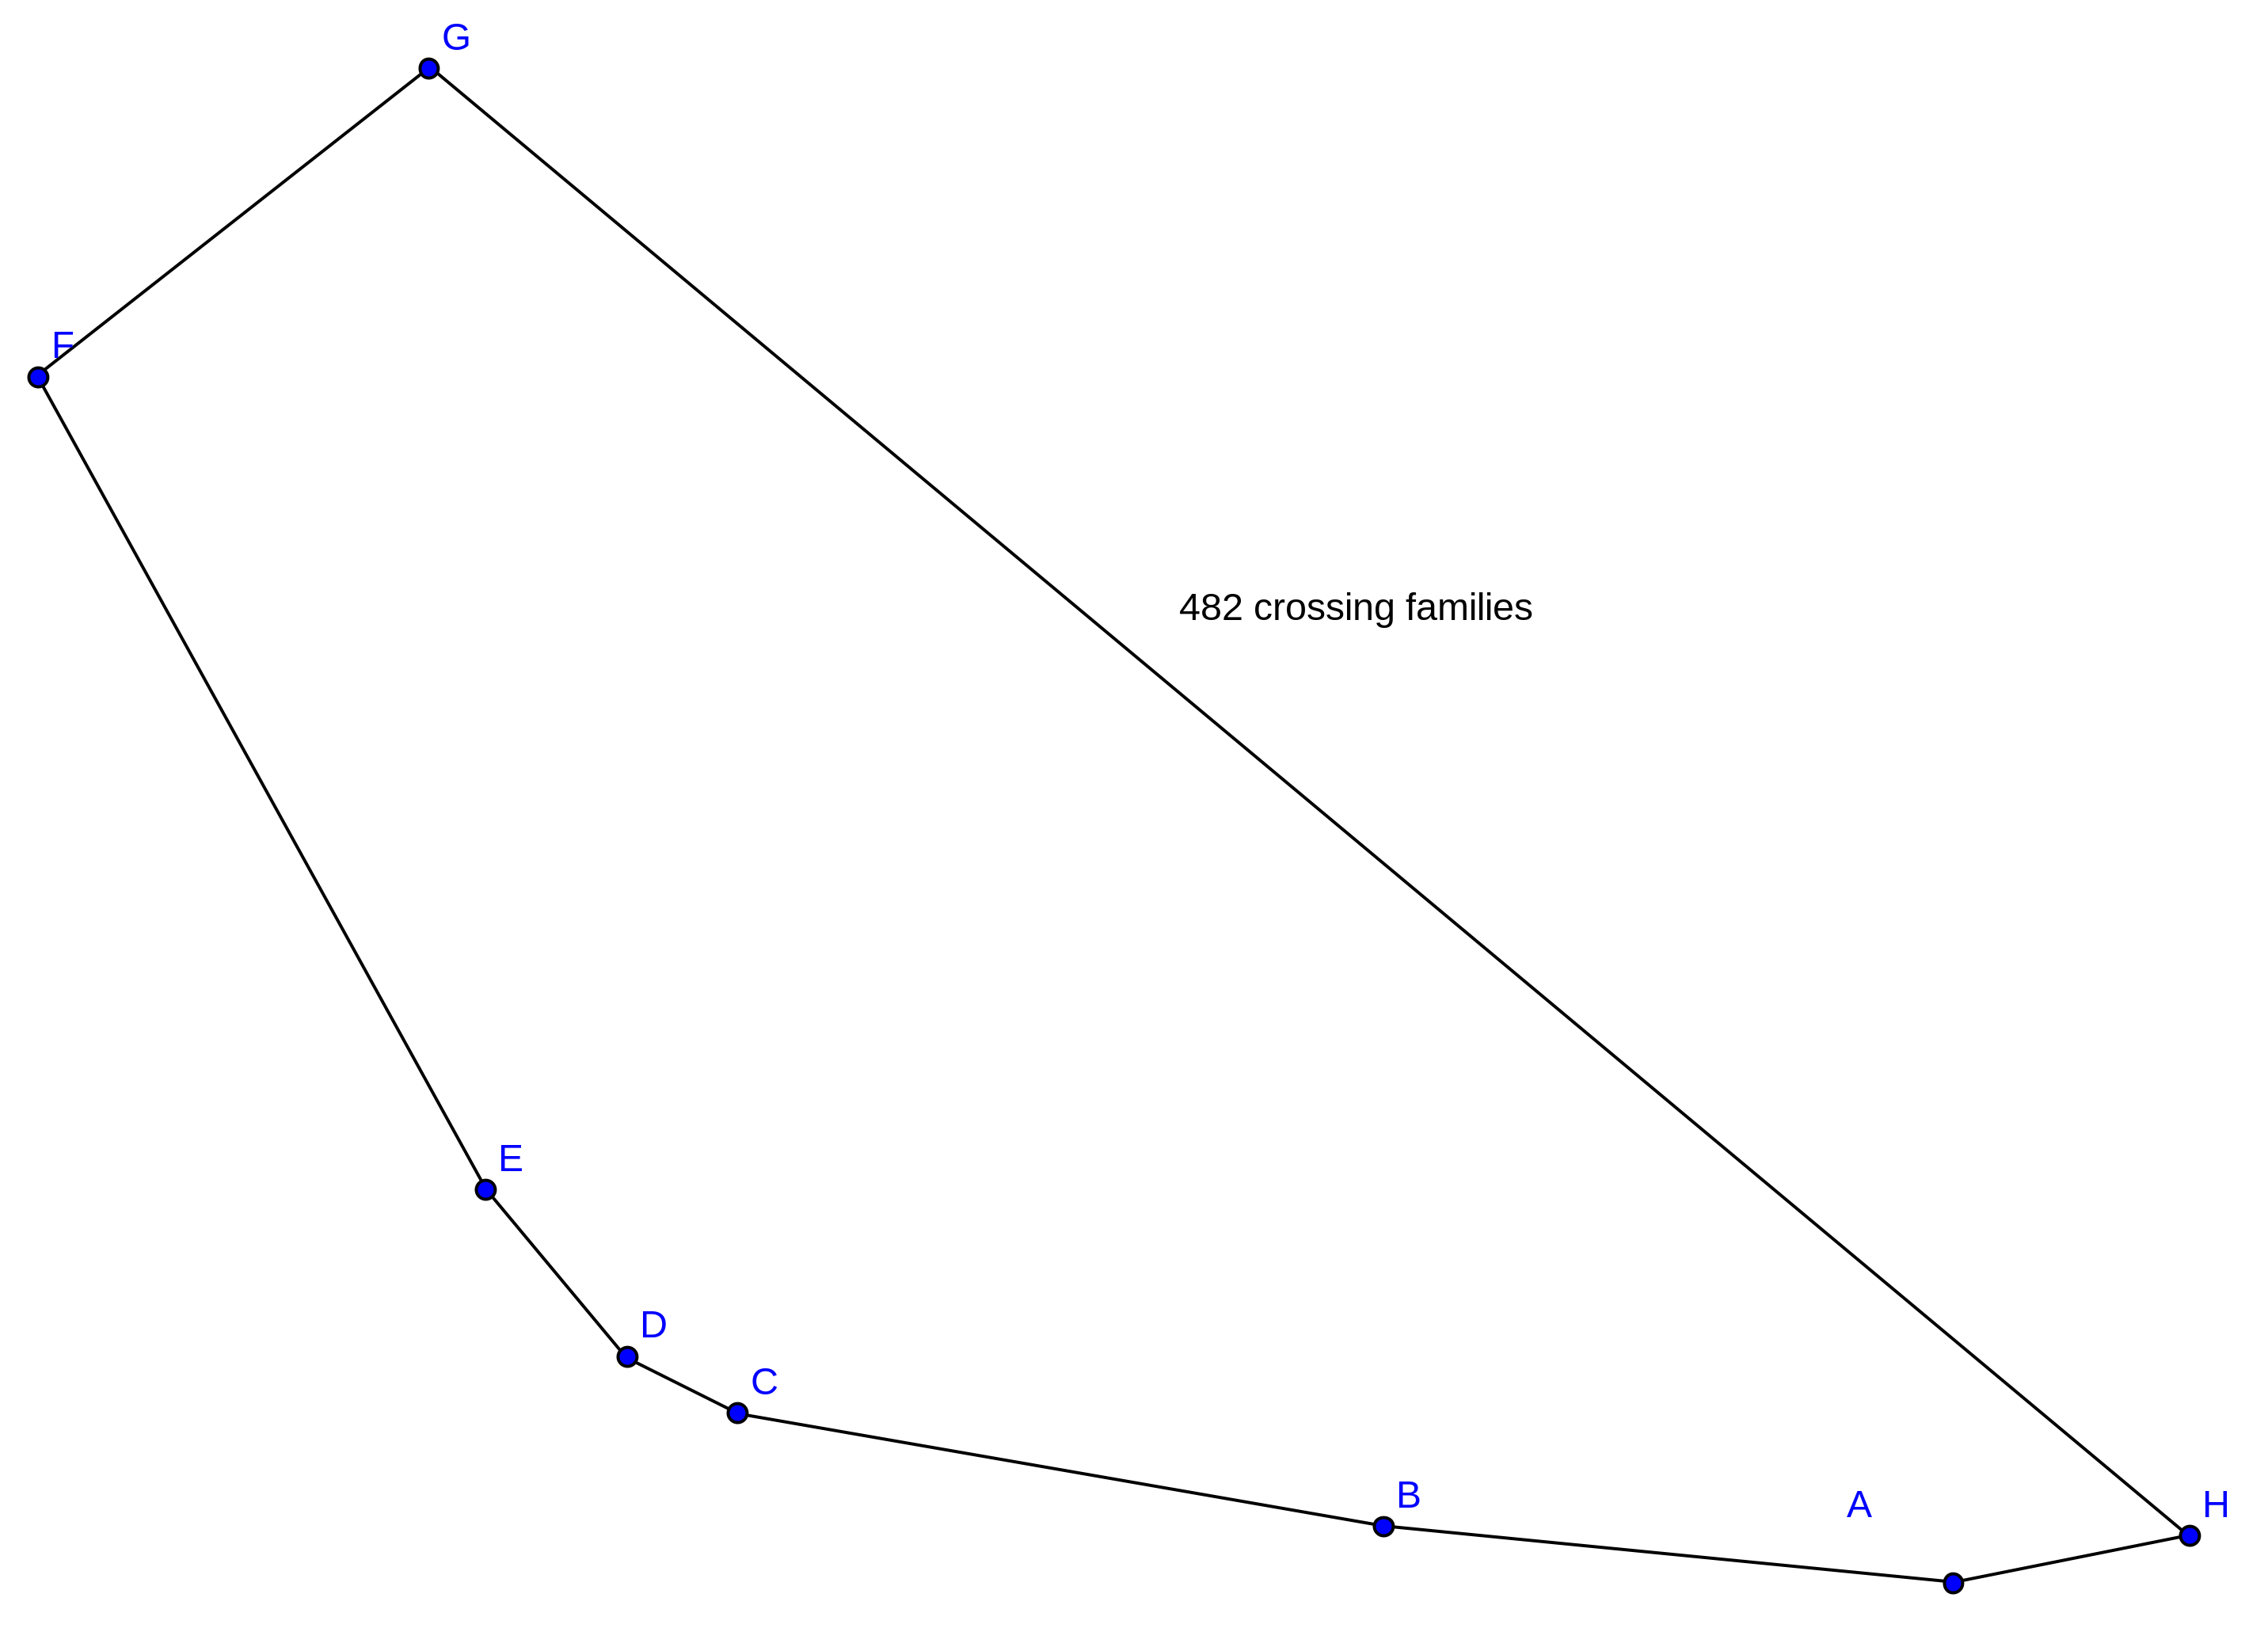
\includegraphics[scale=.25]{2k2/max8_otype1.png}
		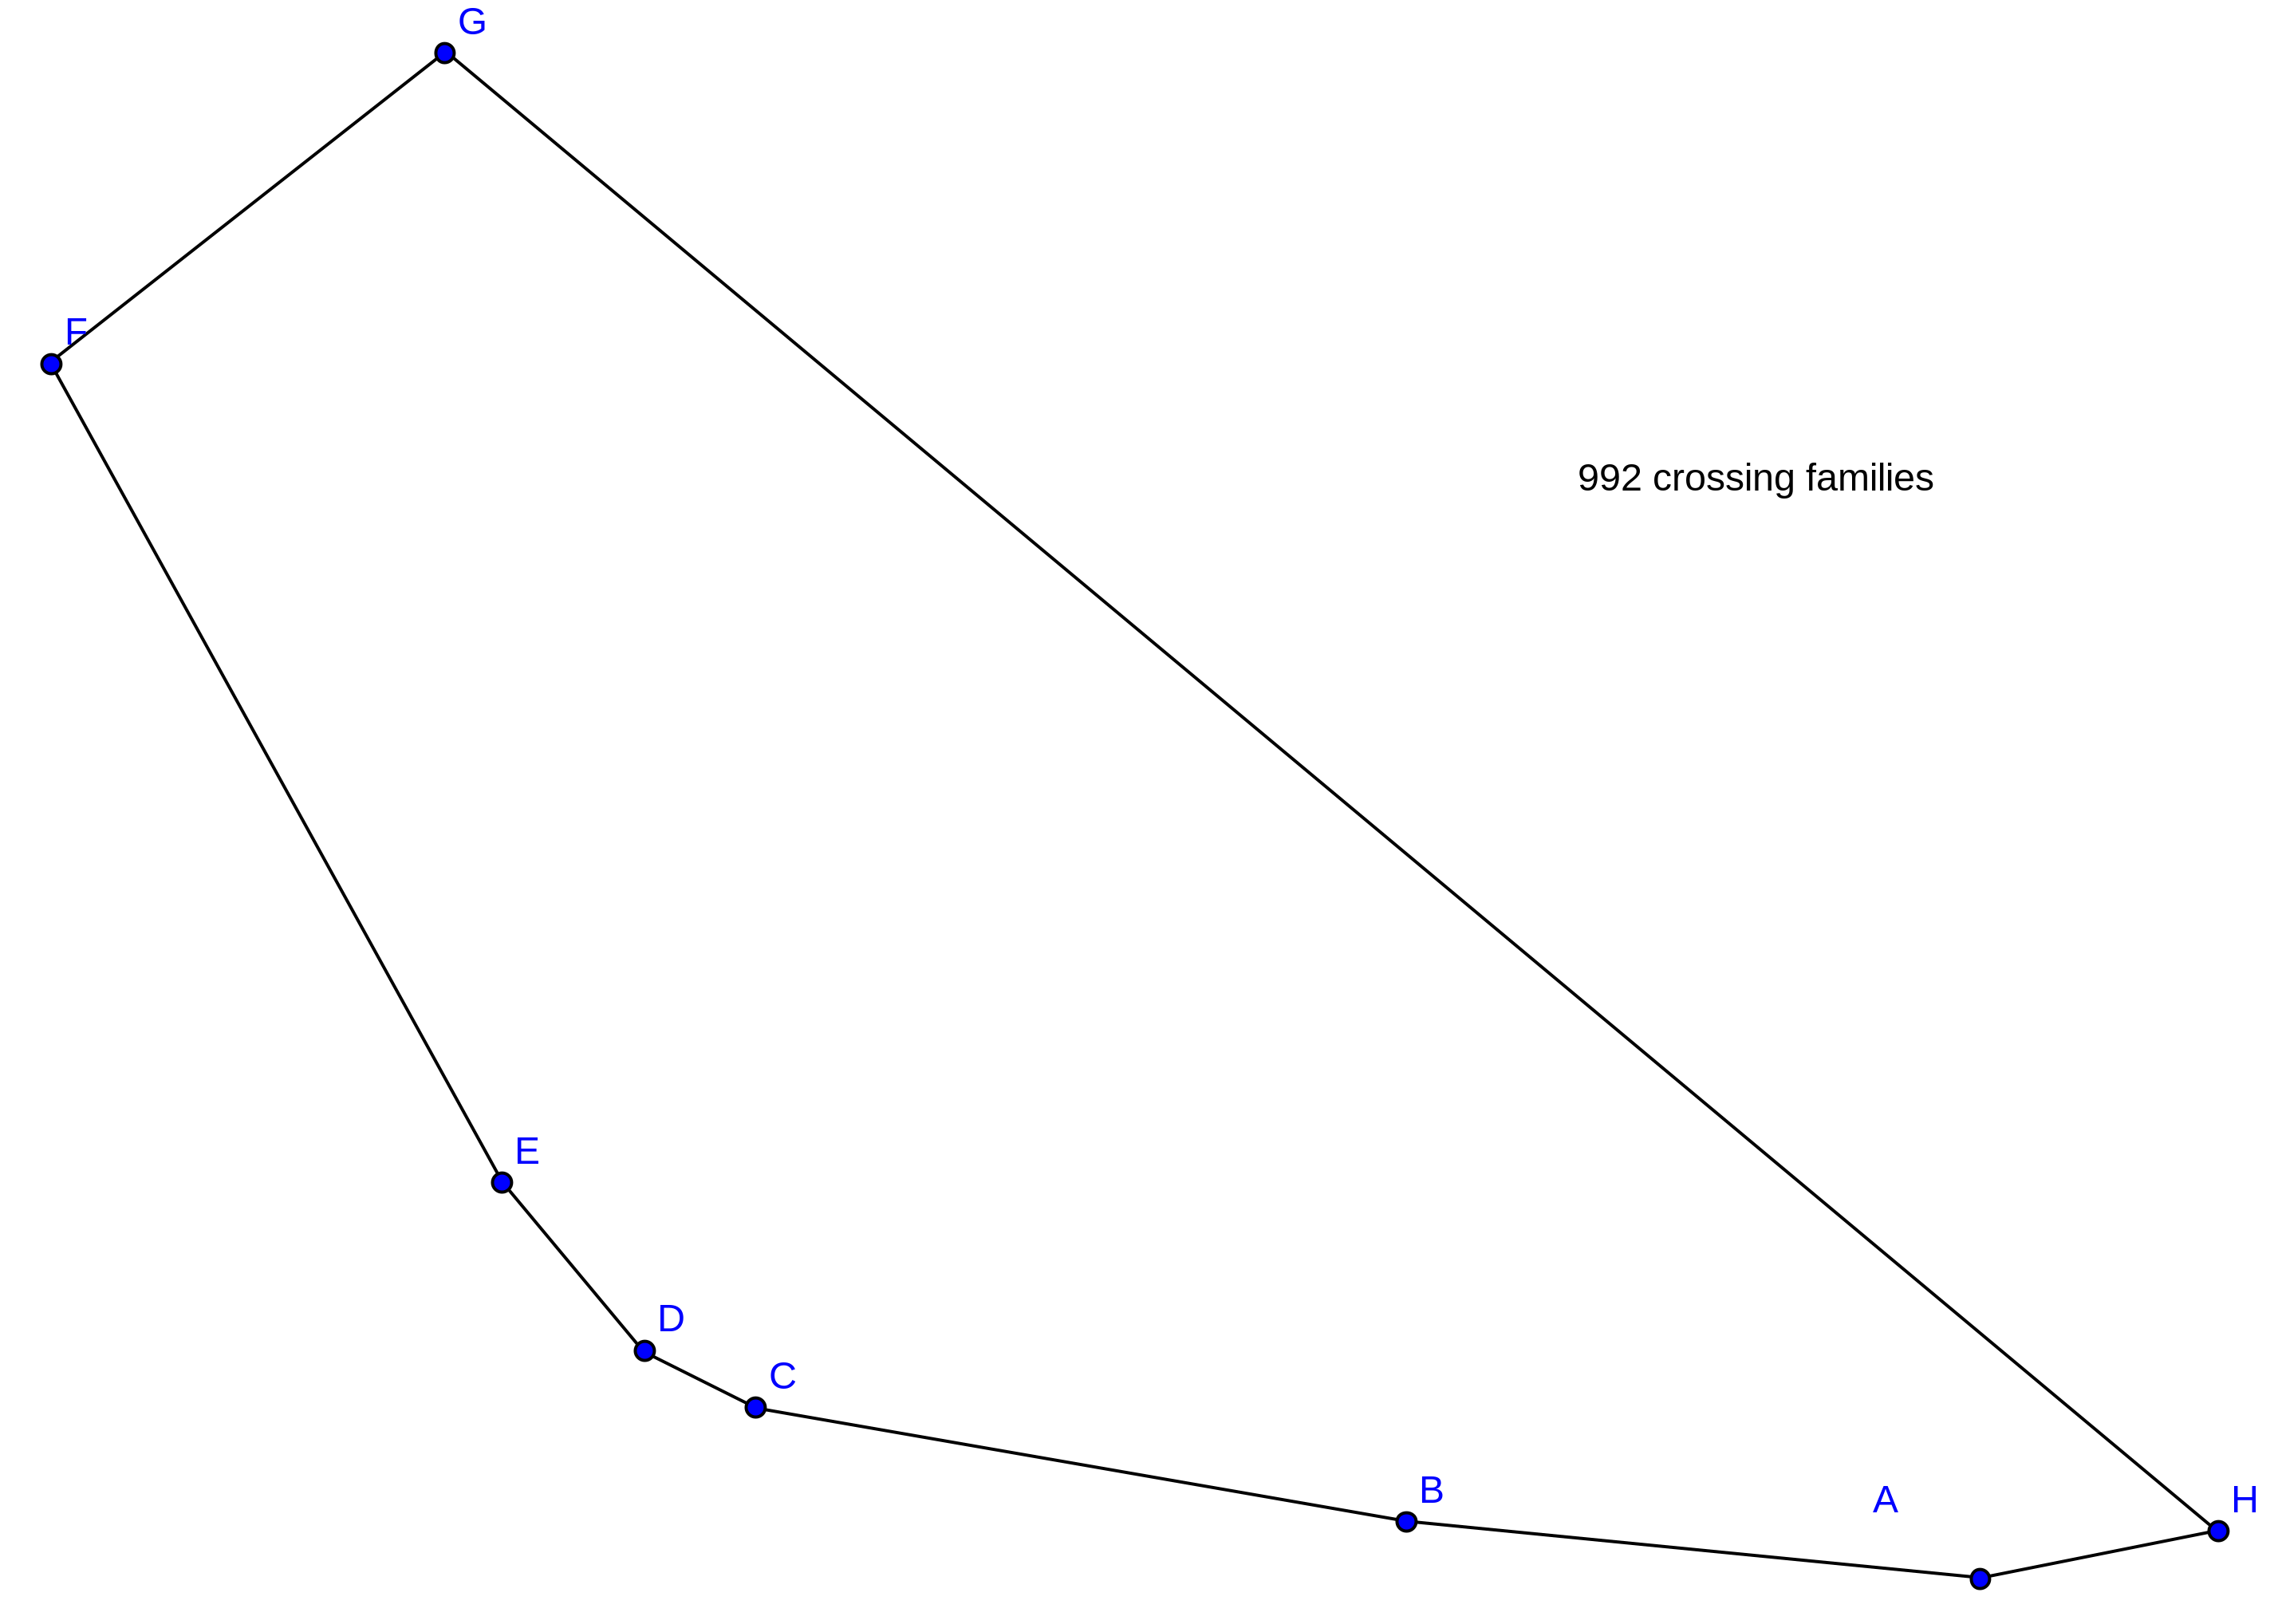
\includegraphics[scale=.25]{k13/max8_otype1.png}
		\caption{otype 1 para $2k2$ y otype 1 para $k_{1,3}$ con 8 puntos}
		
	\end{figure}
	
	\begin{figure}[!h]
		\centering
		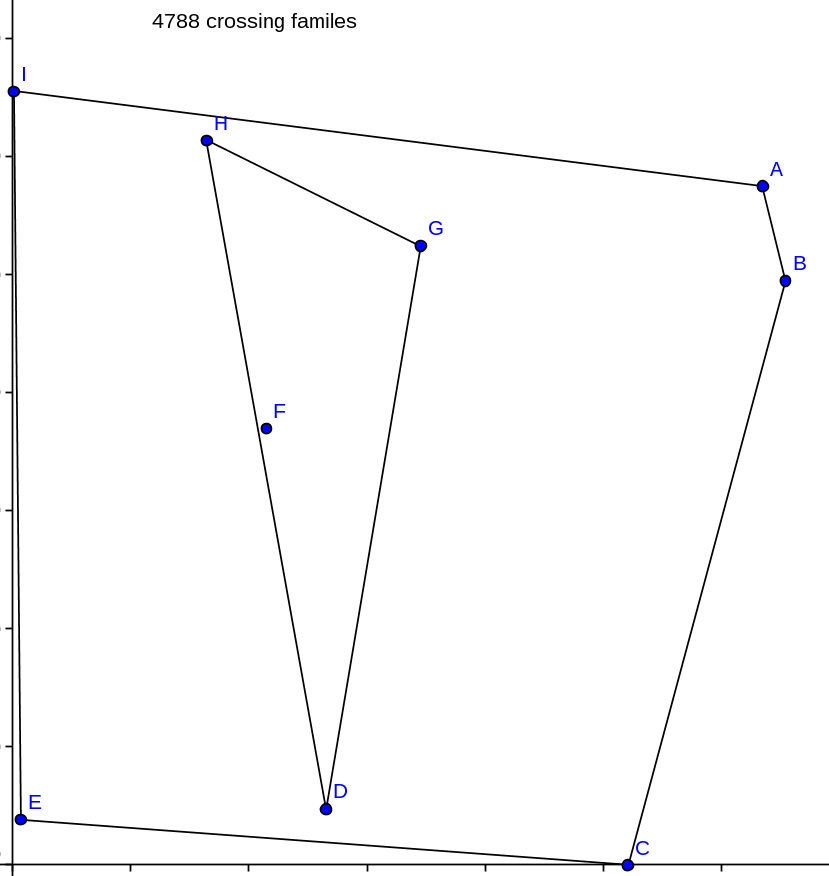
\includegraphics[scale=.65]{2k2/max9_otype5446.png}
		\hspace{10mm}
		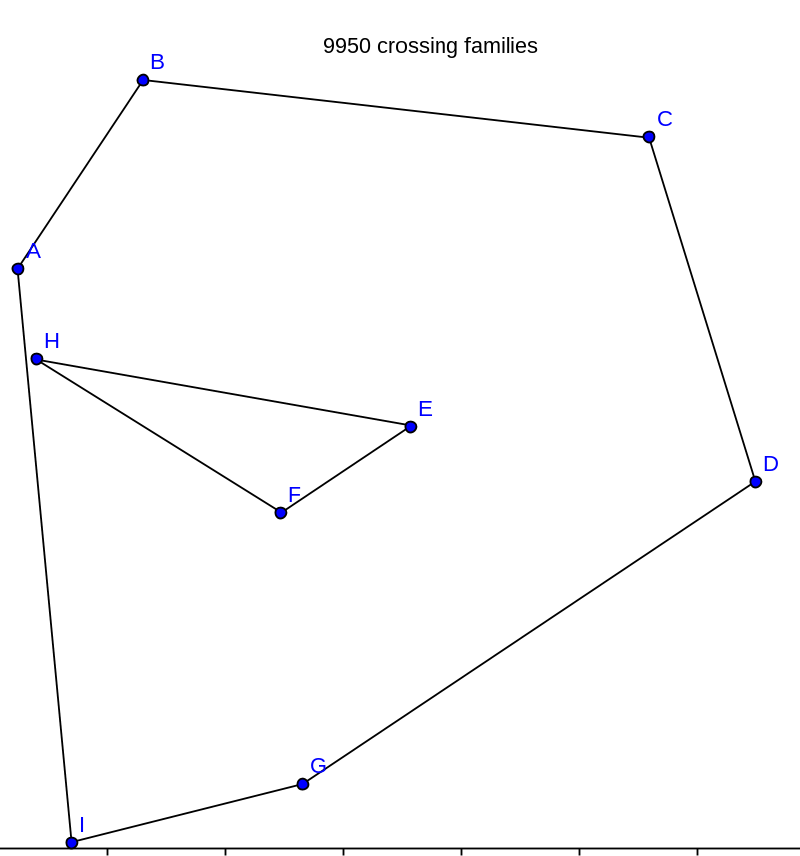
\includegraphics[scale=.65]{k13/max9_otype12327.png}
		\caption{otype 5446 para $2k2$ y otype 12327 para $K_{1,3}$ con 9 puntos}
	\end{figure}	
	
	\begin{figure}[!h]
		\centering
		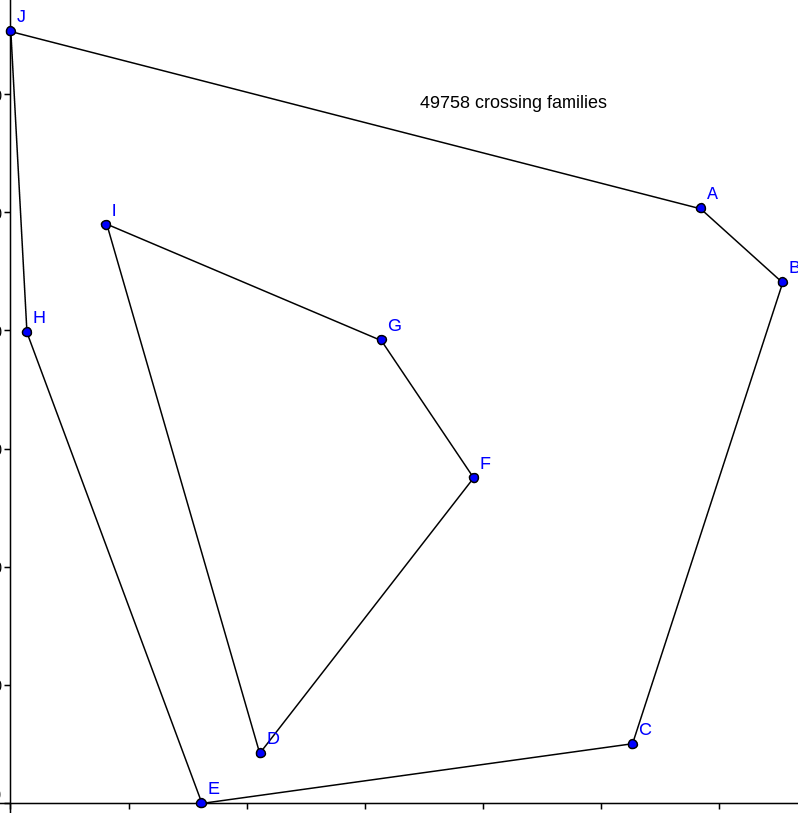
\includegraphics[scale=.7]{k13/max10_otype288026.png}
		\caption{otype 288026 para $K1_3$ con 10 puntos}
	\end{figure}
	
	
\end{document}